

\section{Indledning}
Spillet Galaga er et 2D spil hvor man styrer et rumskib der kan flyve til højre og venstre. Målet er at skyde alle rumvæsnerne inden de når bunden af skærmen. Implementationen vi har lavet er akkumuleret over 3 afleveringer, hvor vi efter hver aflevering har fået feedback. Implementationen af spillet er lavet med en game engine kaldet \texttt{DIKUArcade}. På \autoref{fig:gameplay} ses et screenshot fra vore implementation af Galaga.
\begin{figure}[!ht]
  \center
  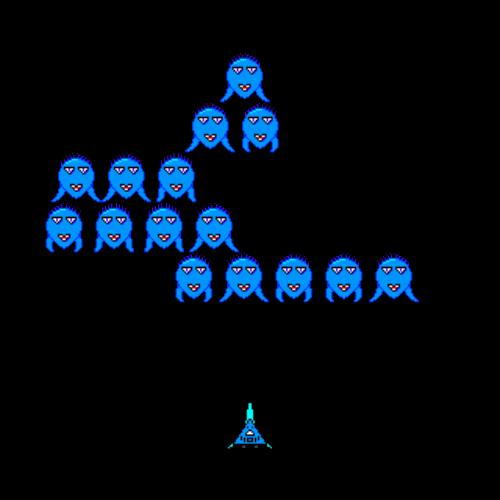
\includegraphics[scale=0.3]{latex/GamePlay}
  \caption{Den sidste implementation af Galaga}
  \label{fig:gameplay}
\end{figure}
\\I løbet af de tre opgaver er implementationen blevet mere og mere omfattende. Efter den første opgave havde vi en implementation der lige nøjagtig var spil-bar. Det vil sige man kunne rykke og skyde, men rumvæsnerne rykkede sig endnu ikke. Efter anden opgave fik vi rumvæsnerne til at bevæge sig og de kunne starte ud i flere forskellige formationer, kaldet squadrons. Nu, efter tredje iteration har vi tilføjet en menu, man kan pause spillet og man taber eller vinder når man hhv. ikke når at skyde rumvæsnerne i tide, eller når at skyde dem alle.
